
\documentclass[12pt,a4paper]{article}
%\usepackage{amsfonts}
%\usepackage{amsmath}
%\usepackage{amsthm}
\usepackage[utf8]{inputenc}
%\usepackage{hyperref}
%\usepackage{booktabs}
\usepackage{graphicx}

\title{Lab 1: Introduction to \texttt{igraph}}
\date{\today}

\begin{document}
\maketitle

\section{Watts--Strotgatz model}

The clustering coefficient $C(p)$ and average shortest path $L(p)$ are computed 
for a Watts--Strotgatz graph with dimension 1, size 200, 4 neighbours and 
probability $p$. Each probability is computed as $p = 2^{-i}$ with $i \in \{0, 
14\}$ (as a logarithmic scale is used). The mean values of 100 random graphs is 
performed to reduce the variance. Also, both are scaled between 0 and 1 to be 
compared using a graph with $p=0$ as $C(p)/C(0)$ and $L(p)/L(0)$.

\begin{center}
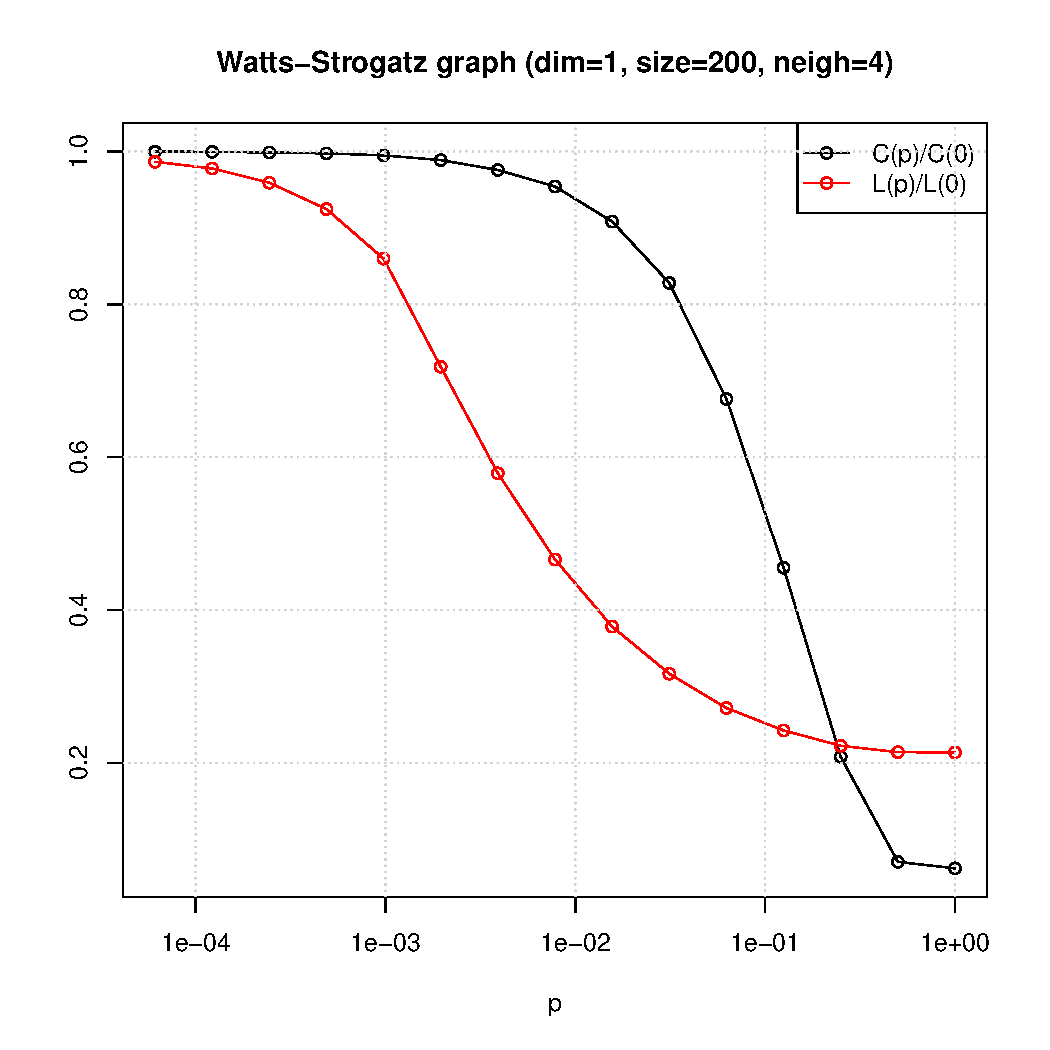
\includegraphics[width=.8\textwidth]{ws.pdf}
\end{center}

\section{Erdös--Rényi model}

The average shortest path is ploted against the number of nodes $n$ of a 
Erdös--Rényi graph. The probability is set as $p = \ln(n)/n$ to keep the graph 
connected. The mean values of 10 random graphs are computed to reduce the 
variance. The number of nodes is kept up to 10000, to maintain a reasonable 
computing time, with $n \in \{500, 1000, \ldots, 10000\}$.

\begin{center}
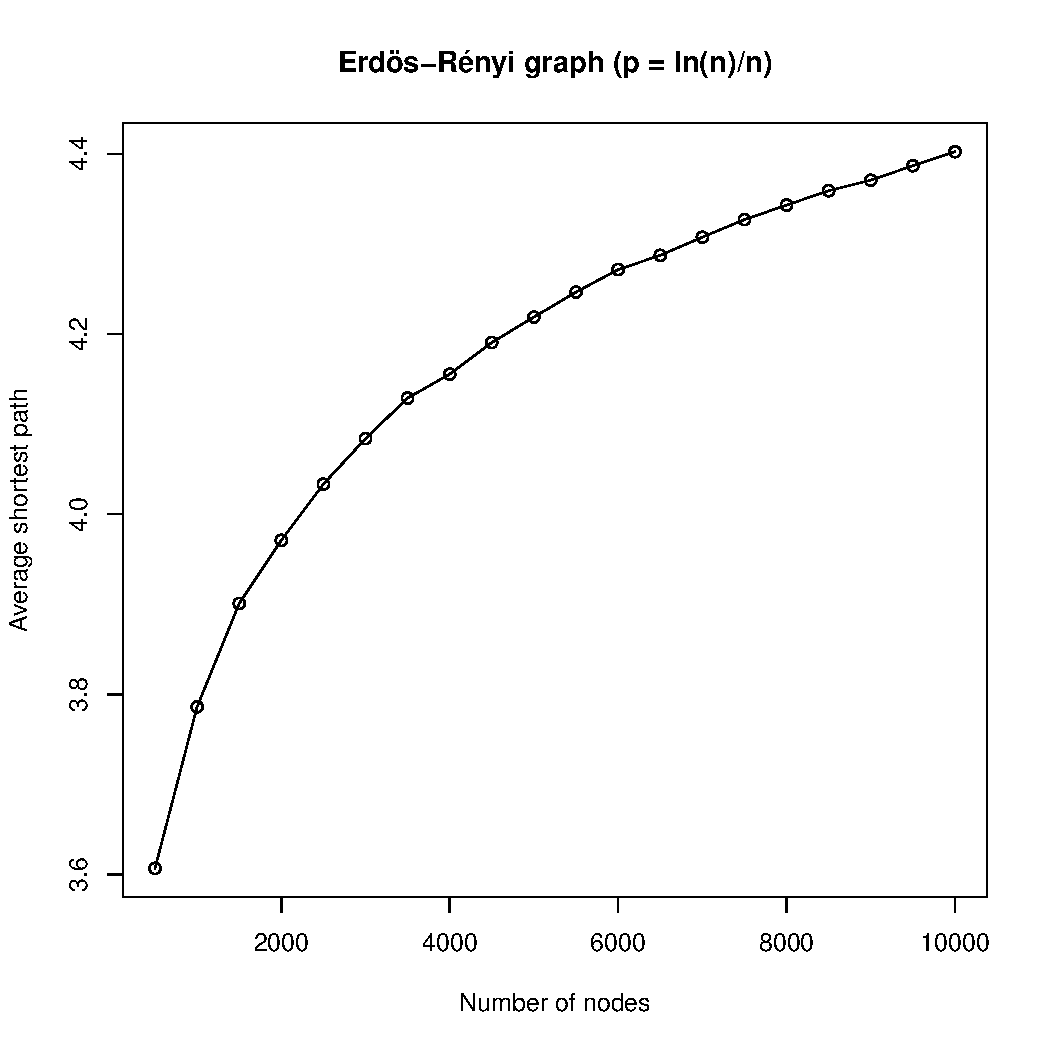
\includegraphics[width=0.8\textwidth]{er.pdf}
\end{center}

\end{document}
